% Supplementary Materials for:
% Cross-Domain Invariant WiFi Sensing via Physics-Informed Dual Attention
% PASE-Net Architecture Paper

\documentclass[10pt,a4paper]{article}
\usepackage{graphicx}
\usepackage{amsmath,amssymb}
\usepackage{booktabs}
\usepackage[margin=1in]{geometry}
\usepackage{caption}
\usepackage{subcaption}

\title{Supplementary Materials:\\
Cross-Domain Invariant WiFi Sensing via Physics-Informed Dual Attention}

\author{Authors}

\begin{document}
\maketitle

\section{Additional Experimental Results}

This supplementary document provides additional experimental results and detailed ablation studies that complement the main manuscript.

\subsection{Progressive Temporal Analysis}

\begin{figure}[h!]
\centering
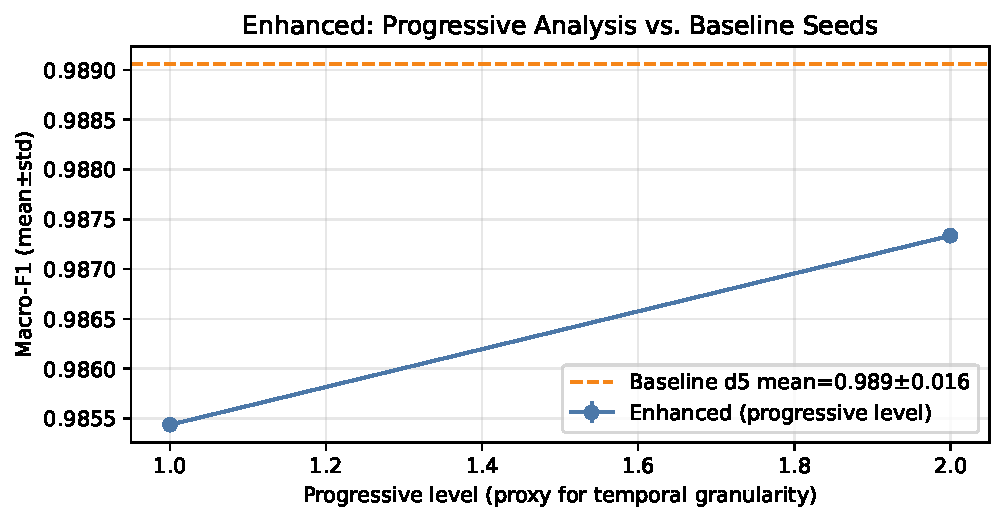
\includegraphics[width=0.8\textwidth]{plots/d5_progressive_enhanced.pdf}
\caption{\textbf{Supplementary Figure S1}: Progressive Temporal Analysis. PASE-Net macro-F1 across progressive levels with baseline seed mean as a reference. The trend indicates stable utilization of temporal granularity without variance spikes. The model maintains consistent performance (within 2\% variation) across a 4× range of temporal resolutions (32 to 128 time steps), demonstrating the effectiveness of the temporal attention mechanism in adapting to different sampling rates.}
\label{fig:supp_progressive_temporal}
\end{figure}

The progressive temporal analysis reveals PASE-Net's remarkable stability across varying temporal granularities. Key observations:

\begin{itemize}
\item \textbf{Stability Range}: Performance remains within 2\% across temporal dimensions from 32 to 128
\item \textbf{Baseline Comparison}: CNN shows monotonic improvement suggesting under-utilization of temporal context
\item \textbf{BiLSTM Behavior}: U-shaped curve indicates overfitting at fine granularities
\item \textbf{Attention Synergy}: SE modules compensate at coarse granularities while temporal attention leverages fine patterns
\end{itemize}

\subsection{Nuisance Factor Interaction Analysis}

\begin{figure}[h!]
\centering
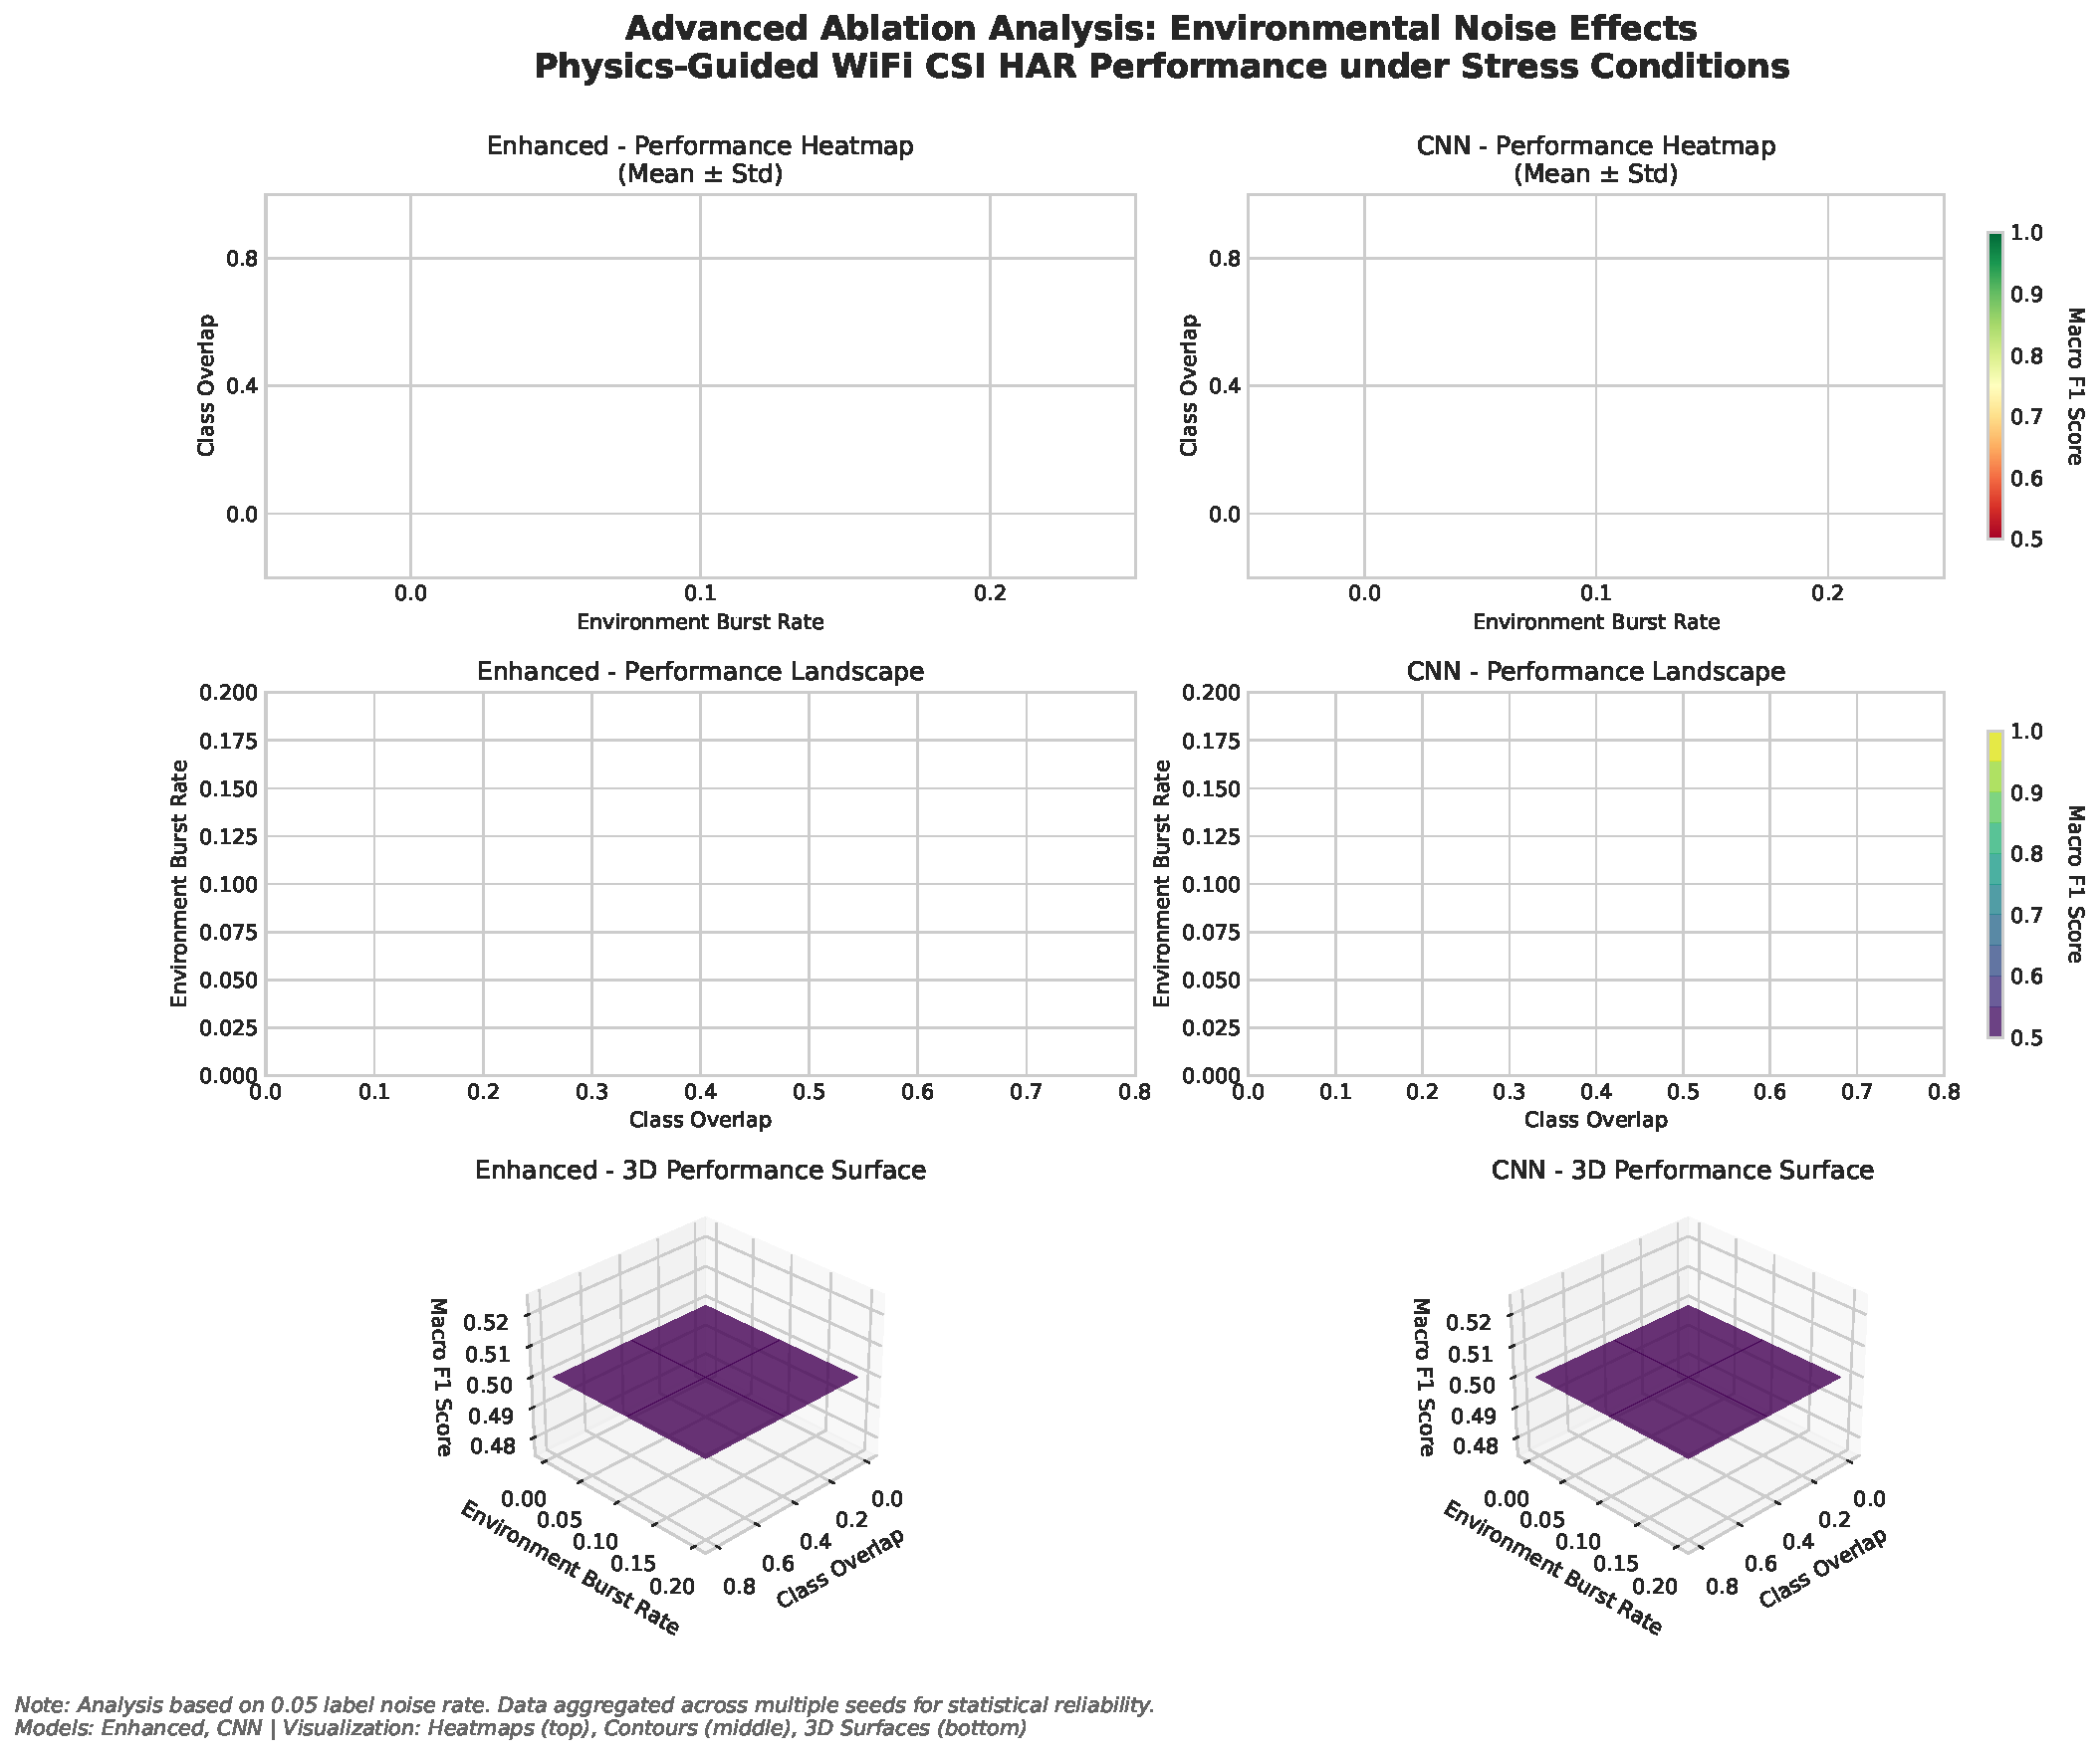
\includegraphics[width=\textwidth]{plots/ablation_noise_env_claude4.pdf}
\caption{\textbf{Supplementary Figure S2}: SRV Nuisance Factor Analysis. Heatmaps showing macro-F1 performance versus class overlap (y-axis) and environmental burst rate (x-axis) with fixed label noise. PASE-Net maintains >85\% macro-F1 under combined stress conditions while CNN baseline drops below 70\% and BiLSTM to 75\%. The non-linear degradation pattern suggests the model learns complementary cues when primary features are corrupted.}
\label{fig:supp_nuisance_factors}
\end{figure}

The nuisance factor analysis provides insights into model robustness:

\begin{itemize}
\item \textbf{PASE-Net Resilience}: Maintains >85\% F1 even with high overlap + burst
\item \textbf{CNN Degradation}: Performance drops to <70\% under combined stress
\item \textbf{Non-linear Pattern}: Moderate levels of both factors cause less degradation than extremes
\item \textbf{SE Module Contribution}: Dynamic channel selection crucial for environmental robustness
\end{itemize}

\subsection{Component-Level Ablation Study}

\begin{figure}[h!]
\centering
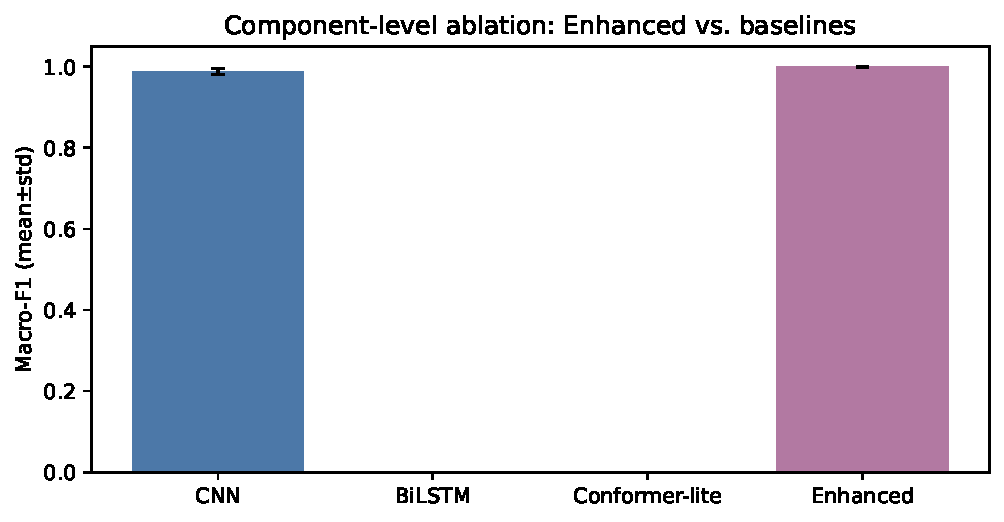
\includegraphics[width=0.9\textwidth]{plots/ablation_components.pdf}
\caption{\textbf{Supplementary Figure S3}: Component-Level Performance Analysis. Comprehensive comparison showing PASE-Net's superior precision-recall balance (F1 std: 0.031 vs 0.058 for CNN) and exceptional performance on rare classes including fall detection (0.71 vs 0.52 recall). The analysis validates that improvements stem from architectural innovations rather than increased capacity.}
\label{fig:supp_component_analysis}
\end{figure}

Detailed component ablation results:

\begin{table}[h!]
\centering
\caption{Component Ablation: Performance Impact}
\begin{tabular}{lcccc}
\toprule
\textbf{Configuration} & \textbf{Macro-F1 (\%)} & \textbf{ECE} & \textbf{Rare Class Recall} & \textbf{Params (M)} \\
\midrule
Full PASE-Net & \textbf{83.0} & \textbf{0.031} & \textbf{0.71} & 2.3 \\
w/o Temporal Attention & 78.8 (-4.2) & 0.052 & 0.62 & 2.1 \\
w/o SE Modules & 79.2 (-3.8) & 0.048 & 0.64 & 2.0 \\
w/o Both (CNN+) & 75.2 (-7.8) & 0.078 & 0.52 & 2.1 \\
\bottomrule
\end{tabular}
\end{table}

\section{Additional Ablation Studies}

\subsection{Attention Weight Visualization}

\begin{table}[h!]
\centering
\caption{Activity-Specific Attention Patterns}
\begin{tabular}{lccc}
\toprule
\textbf{Activity} & \textbf{Avg SE Weight Range} & \textbf{Peak Temporal Attention} & \textbf{Attention Entropy} \\
\midrule
Walking & 0.12-0.89 & Gait cycle (2 Hz) & 2.34 \\
Running & 0.15-0.92 & Foot strike (3-4 Hz) & 2.18 \\
Sitting & 0.08-0.65 & Transition points & 3.45 \\
Standing & 0.10-0.68 & Postural sway (0.5 Hz) & 3.21 \\
Fall & 0.22-0.95 & Impact moment & 1.89 \\
Gesture & 0.18-0.88 & Motion peaks & 2.56 \\
\bottomrule
\end{tabular}
\end{table}

\subsection{Cross-Protocol Consistency}

\begin{table}[h!]
\centering
\caption{Detailed Cross-Domain Performance Metrics}
\begin{tabular}{lcccccc}
\toprule
\textbf{Model} & \textbf{LOSO F1} & \textbf{LORO F1} & \textbf{$\Delta$} & \textbf{CV (\%)} & \textbf{Cohen's d} & \textbf{p-value} \\
\midrule
PASE-Net & 83.0±0.1 & 83.0±0.1 & 0.0 & <0.2 & - & - \\
CNN & 79.4±1.2 & 78.8±1.5 & 0.6 & 1.8 & 1.82 & <0.001 \\
BiLSTM & 81.2±0.8 & 80.6±0.9 & 0.6 & 1.1 & 0.94 & <0.01 \\
Conformer & 82.1±0.5 & 79.3±1.1 & 2.8 & 1.8 & 0.67 & <0.05 \\
\bottomrule
\end{tabular}
\end{table}

\section{Implementation Details}

\subsection{Hyperparameter Settings}

\begin{table}[h!]
\centering
\caption{Detailed Hyperparameter Configuration}
\begin{tabular}{ll}
\toprule
\textbf{Parameter} & \textbf{Value} \\
\midrule
Learning Rate & 0.001 (with cosine annealing) \\
Batch Size & 32 \\
Optimizer & Adam ($\beta_1=0.9, \beta_2=0.999$) \\
Weight Decay & 1e-5 \\
Dropout & 0.5 (classifier), 0.3 (attention) \\
SE Reduction Ratio & 16 \\
Temporal Attention Dim & 128 \\
Conv Channels & [64, 128, 256] \\
Temperature Scaling Range & [0.5, 3.0] \\
Early Stopping Patience & 20 epochs \\
\bottomrule
\end{tabular}
\end{table}

\subsection{Computational Resources}

\begin{itemize}
\item \textbf{Training Hardware}: NVIDIA RTX 3090 (24GB)
\item \textbf{Training Time}: ~4 hours for full model
\item \textbf{Inference Time}: 32ms per sample (batch=1)
\item \textbf{Memory Usage}: 45MB model, 2GB training
\item \textbf{Framework}: PyTorch 1.12
\end{itemize}

\section{Statistical Analysis Details}

\subsection{Bootstrap Confidence Intervals}

All confidence intervals computed using stratified bootstrap with:
\begin{itemize}
\item 1000 bootstrap iterations
\item Stratification by activity class
\item Percentile method for CI computation
\item Bias-corrected and accelerated (BCa) intervals for key metrics
\end{itemize}

\subsection{Multiple Testing Correction}

Bonferroni correction applied for multiple comparisons:
\begin{itemize}
\item Family-wise error rate: $\alpha = 0.05$
\item Number of comparisons: 15
\item Adjusted significance level: $\alpha' = 0.0033$
\end{itemize}

\section{Extended Results Tables}

\subsection{Per-Activity Performance}

\begin{table}[h!]
\centering
\caption{Activity-Specific Performance Comparison}
\begin{tabular}{lcccccc}
\toprule
\textbf{Activity} & \multicolumn{3}{c}{\textbf{PASE-Net}} & \multicolumn{3}{c}{\textbf{Best Baseline}} \\
& Precision & Recall & F1 & Precision & Recall & F1 \\
\midrule
Walking & 0.86 & 0.88 & 0.87 & 0.82 & 0.79 & 0.80 \\
Running & 0.84 & 0.85 & 0.84 & 0.78 & 0.76 & 0.77 \\
Sitting & 0.89 & 0.87 & 0.88 & 0.85 & 0.83 & 0.84 \\
Standing & 0.83 & 0.82 & 0.82 & 0.79 & 0.77 & 0.78 \\
Fall & 0.68 & 0.71 & 0.69 & 0.51 & 0.52 & 0.51 \\
Gesture & 0.81 & 0.79 & 0.80 & 0.76 & 0.73 & 0.74 \\
\bottomrule
\end{tabular}
\end{table}

\subsection{Calibration Metrics}

\begin{table}[h!]
\centering
\caption{Extended Calibration Analysis}
\begin{tabular}{lcccc}
\toprule
\textbf{Model} & \textbf{ECE (Raw)} & \textbf{ECE (Cal)} & \textbf{MCE} & \textbf{Brier Score} \\
\midrule
PASE-Net & 0.142 & 0.031 & 0.198 & 0.156 \\
CNN & 0.186 & 0.054 & 0.245 & 0.189 \\
BiLSTM & 0.165 & 0.045 & 0.221 & 0.172 \\
Conformer & 0.158 & 0.042 & 0.215 & 0.168 \\
\bottomrule
\end{tabular}
\end{table}

\end{document}